\documentclass[11pt]{article}
\usepackage[letterpaper,margin=.25in]{geometry}
\usepackage{amsmath,amssymb,booktabs,array,tabularx,xcolor,tikz,hyperref,embedfile,microtype}
\usetikzlibrary{trees}
\hypersetup{colorlinks=true,urlcolor=blue!55!black}
\pagestyle{empty}
\setlength{\parindent}{0pt}
\setlength{\parskip}{4pt}
\linespread{1.035}\selectfont
\definecolor{navy}{RGB}{25,54,86}
\definecolor{soft}{RGB}{244,247,250}
\tikzset{branch/.style={circle,draw=navy,line width=.6pt,inner sep=2pt},trueleaf/.style={circle,draw=navy,fill=navy,inner sep=2.1pt},falseleaf/.style={circle,draw=navy,fill=white,inner sep=1.8pt}}
\newcommand{\sectionbar}[1]{\vspace{3pt}{\color{navy}\bfseries #1}\par\vspace{2pt}\hrule\vspace{4pt}}
\begin{document}
\enlargethispage{.12in}

\embedfile[desc={A120594 exact certificate payload},mimetype=application/json]{certificate_payload.json}
{\color{navy}\LARGE\bfseries A120594 concise calculus certificate}\hfill{\small VERIFIED}\\[-1pt]
{\small Bradley Klee, \quad Mech.An.ika Sol (Open AI) \hfill July 31, 2026}

\sectionbar{Definition and first terms}
\(\displaystyle 8\,A(x)=7+8\,x+A(x)^{4}\), with the origin-normalized solution.\\
{\footnotesize Normalization/grammar: \texttt{A(x)=1+(2)*T(x); T=x+3*T\textasciicircum{}2+4*T\textasciicircum{}3+2*T\textasciicircum{}4}.}\\
\(a(0),\ldots,a(7)=1,2,6,44,394,3948,42364,476120\).\\[2pt]
{\small Kernel used throughout: \(\displaystyle \rho(u)=u\,(1-3\,u^{1}-4\,u^{2}-2\,u^{3})\), so \(x=\rho(T(x))\).}

\sectionbar{Typogeometry}
\begin{minipage}[t]{.235\textwidth}\centering 
\begin{tikzpicture}[level distance=9mm,level 1/.style={sibling distance=10mm},level 2/.style={sibling distance=6mm},scale=.82,transform shape] \node[trueleaf] (n0) {};\end{tikzpicture}\\[2pt]{\normalsize\texttt{1x2}}\end{minipage}\begin{minipage}[t]{.235\textwidth}\centering 
\begin{tikzpicture}[level distance=9mm,level 1/.style={sibling distance=10mm},level 2/.style={sibling distance=6mm},scale=.82,transform shape] \node[branch,fill=orange!24] (n0) {} child {node[trueleaf] (n1) {}} child {node[trueleaf] (n2) {}};\end{tikzpicture}\\[2pt]{\normalsize\texttt{\{1,1\}x6}}\end{minipage}\begin{minipage}[t]{.235\textwidth}\centering 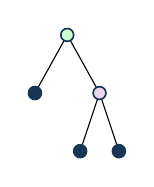
\begin{tikzpicture}[level distance=9mm,level 1/.style={sibling distance=10mm},level 2/.style={sibling distance=6mm},scale=.82,transform shape] \node[branch,fill=green!20] (n0) {} child {node[trueleaf] (n1) {}} child {node[branch,fill=violet!16] (n2) {} child {node[trueleaf] (n3) {}} child {node[trueleaf] (n4) {}}};\end{tikzpicture}\\[2pt]{\normalsize\texttt{\{1,\{1,1\}\}x18}}\end{minipage}\begin{minipage}[t]{.235\textwidth}\centering 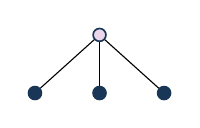
\begin{tikzpicture}[level distance=9mm,level 1/.style={sibling distance=10mm},level 2/.style={sibling distance=6mm},scale=.82,transform shape] \node[branch,fill=violet!16] (n0) {} child {node[trueleaf] (n1) {}} child {node[trueleaf] (n2) {}} child {node[trueleaf] (n3) {}};\end{tikzpicture}\\[2pt]{\normalsize\texttt{\{1,1,1\}x8}}\end{minipage}

{\footnotesize colored arity geometry; node color distinguishes constructors. Filled endpoints are true leaves; open endpoints are false/empty leaves. For colored grammars, color is genuine constructor data and is not silently converted into a positional zero pattern.}

{\footnotesize Typogeometric constructor codes and multiplicities: \(\Delta_{2}\!:\,3,\;\Delta_{3}\!:\,4,\;\Delta_{4}\!:\,2\).}

\sectionbar{Coefficient and contour extraction}
{\footnotesize \[\begin{gathered}\mathcal K_n=\{(k_1,\ldots,k_3)\in\mathbb Z_{\ge0}^{3}:\sum_{j=1}^{3}jk_j=n-1\},\quad K=\sum_{j=1}^{3}k_j,\\a(n)=\frac{2}{n}\sum_{\boldsymbol k\in\mathcal K_n}\binom{n+K-1}{K}\binom{K}{k_1,\ldots,k_3}3^{k_1} 4^{k_2} 2^{k_3}.\end{gathered}\]}
\(a(n)=\dfrac{2}{2\pi i n}\oint_\gamma\dfrac{du}{\rho(u)^n},\quad n\ge1.\)

\sectionbar{Recurrence}
{\footnotesize \(\sum_{r=0}^{3}P_r(n)a(n+r)=0\), \(n\ge 1\), with \[\begin{aligned}P_{0}(n)&=-512\,n^{3} - 768\,n^{2} - 96\,n + 80\\P_{1}(n)&=-1344\,n^{3} - 4032\,n^{2} - 3892\,n - 1204\\P_{2}(n)&=-1176\,n^{3} - 5292\,n^{2} - 7644\,n - 3528\\P_{3}(n)&=89\,n^{3} + 534\,n^{2} + 979\,n + 534\end{aligned}\]}

\sectionbar{Differential equation}
{\footnotesize \[\begin{aligned}&\left(80\,x^{3}\right)A(x)+\left(-1376\,x^{4} - 1204\,x^{3}\right)A'(x)\\[-1pt]&+\left(-2304\,x^{5} - 4032\,x^{4} - 1764\,x^{3}\right)A^{(2)}(x)+\left(-512\,x^{6} - 1344\,x^{5} - 1176\,x^{4} + 89\,x^{3}\right)A^{(3)}(x)=0.\end{aligned}\]}

\sectionbar{Matrices, telescoper certificate, and checks}
\begingroup\renewcommand{\arraystretch}{1.42}\setlength{\arraycolsep}{5pt}{\small\[\displaystyle U=\begin{pmatrix}\frac{1016}{89}&\frac{144}{89}&\frac{12}{89}&\frac{1}{89}\\\frac{1824}{89}&\frac{152}{89}&\frac{72}{89}&\frac{6}{89}\\\frac{1152}{89}&\frac{96}{89}&\frac{8}{89}&\frac{60}{89}\\0&0&0&0\end{pmatrix},\quad V=\begin{pmatrix}-1&0&0&0\\\frac{482}{89}&\frac{55}{89}&\frac{12}{89}&\frac{1}{89}\\\frac{600}{89}&\frac{50}{89}&\frac{19}{89}&\frac{9}{89}\\\frac{288}{89}&\frac{24}{89}&\frac{2}{89}&\frac{15}{89}\end{pmatrix},\quad J=\begin{pmatrix}0&1&0&0\\0&0&2&0\\0&0&0&3\\0&0&0&0\end{pmatrix}\]}\endgroup
\par\vspace{6pt}
{\small\textbf{Certificate.}\par\smallskip\(\displaystyle R(n,u)=N(n,u)/\rho(u)^{2},\ \deg_uN=9.\)\par}
\vspace{4pt}
{\small Telescoping identity: \(\sum_r P_r(n)H_{n+r}(u)=\partial_u\!\left(R(n,u)H_n(u)\right).\)\par}
\vspace{4pt}
{\footnotesize Matrix dimensions: \(8\times 8\); remainder \(3\times 4\), rank 3, nullity 1. The exact telescoping residual is zero. The recurrence reconstructs all 24 stored terms; 6/6 published OEIS prefix terms match.\par}

\vfill
\colorbox{soft}{\parbox{.97\textwidth}{\tiny Canonical records: \texttt{data/tree\_model.json}, \texttt{data/contour.json}, \texttt{data/matrices.json}, \texttt{data/recurrence.json}, \texttt{data/ode.json}. Embedded payload contains exact sources and SHA-256 matrix identifiers. Compare with the verbose certificate for A120590.}}
\end{document}
